\chapter{绪论}
\label{cha:intro}

\section{引言}

\section{主要工作}

\subsection{基于百科模板的跨语言属性对齐}
\subsection{大规模中英文跨语言知识库XLore的构建}
\subsection{XLore系统与应用接口构建}

\section{主要贡献}
本文提出了一种领域模板生成与领域跨语言属性对齐的方法,并利用对齐结果与四个百科数据源的抽取结果,构建通用领域的中英文知识库XLore,其中主要贡献列举如下:
\begin{itemize}
\item {\heiti 1) 领域模板下的跨百科跨语言属性对齐,} 工程抽取与算法计算相结合,提取出英文维基百科与百度百科两个异构百科下的信息框属性关系。包括百科下属性模板生成,与限定领域下的中英文属性匹配。该方法在构建大规模知识库过程中,对于从多语言的异构数据源生成对齐的shema有一定的贡献。
\item {\heiti 2) 构建了通用领域的跨语言知识库XLore,} 融合基于不同语言的异构百科,获取语义信息,解决中英文知识数量不平衡的问题,该知识库是当前大规模的中英文知识库之一,在跨语言语义网络上有着无限的应用潜能。
\item {\heiti 3) 提供了便于数据访问的可视化系统与应用接口,}前者分别从一般用户与专业用户的不同角度,给出搜索框查询与SPQARQL查询两种知识访问方式;后者考虑知识库的应用场景,提供基于RestFul的实体访问API,对给定文本进行实体分析与排歧,返回实体语义信息,实现了一定应用价值。
\end{itemize}

\section{论文组织}

本文通过绪论、研究现状、基于百科模板的跨语言属性对齐、大规模中英文跨语言知识库XLore的构建、XLore系统与应用接口、总结与展望共6个章节来组织全文内容,其章节关系与结构组织如图\ref{fig:organization}所示:

\begin{figure}[H] % use float package if you want it here
  \centering
  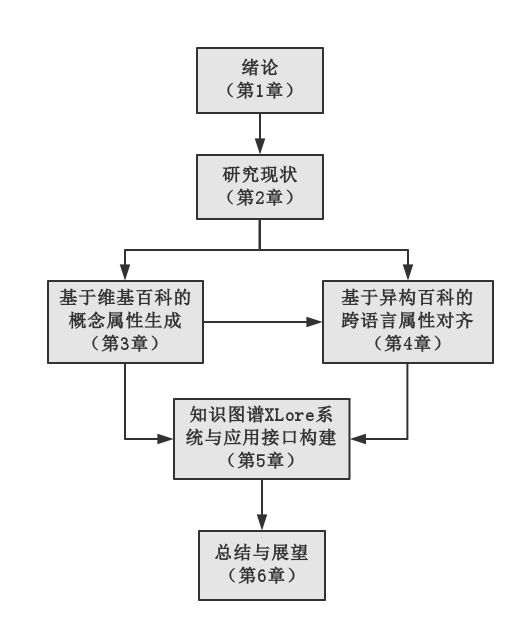
\includegraphics[width=0.5\columnwidth]{organization}
  \caption{论文组织结构图}
  \label{fig:organization}
\end{figure}

第 1 章为绪论,对本文的研究背景进行描述,概要地介绍工作内容,并交待论文的主要贡献及文章组织结构;

第 2 章为研究现状,对当前构建跨语言知识图谱过程的跨语言对齐研究现状进行描述,包括实例对齐、属性对齐,此外列举当前广为人知多语言知识图谱与中文知识图谱,并介绍其构建技术;

第 3 章描述了基于百科模板的跨语言属性对齐流程。首先通过观察与抽取百科中的模板与属性,获得初始的属性集合,之后进行领域模板生成的分析,并实现在特定领域下,同语言相似属性的对齐与跨语言属性链接;

第 4 章介绍了基于在线百科,构建跨语言知识图谱的过程。该工作从中英文维基百科、百度百科、互动百科中抽取语义数据与跨语言关系,并复用第3章的研究结果,对齐中英文知识,致力于解决中英文知识不平衡问题;

第 5 章介绍了基于第4章构建的知识库而搭建的可视化系统与数据访问接口,从实际应用角度展示XLore知识库的结构化与可用性;

第 6 章对本文提出的跨语言属性对齐与知识图谱构造研究工作进行了总结和展望,分析了不足之处,为下一步研究提出了新的建议和意见。
 

